\documentclass[conference]{IEEEtran}

\usepackage[utf8]{inputenc}
\usepackage[T1]{fontenc}
\usepackage{amsmath,amssymb,amsfonts}
\usepackage{graphicx}
\usepackage{booktabs}
\usepackage{tabularx}
\usepackage{ragged2e}
\usepackage{multirow}
\usepackage{cite}
\usepackage{url}
\usepackage{textcomp}
\usepackage{xcolor}
\usepackage{hyperref}
\usepackage{orcidlink}

\hypersetup{colorlinks=false, pdfborder={0 0 0}}

% Full-width table columns:
% J = a stretchable, fully justified text column.
% C = a stretchable, centered column for compact headings and numeric values.
\newcolumntype{J}{>{\justifying\arraybackslash}X}
\newcolumntype{C}{>{\centering\arraybackslash}X}


% Compact spacing to keep the paper within the six-page limit.
% These settings change only layout, not the paper text.
\setlength{\textfloatsep}{5pt plus 1pt minus 2pt}
\setlength{\floatsep}{4pt plus 1pt minus 2pt}
\setlength{\intextsep}{5pt plus 1pt minus 2pt}
\setlength{\abovecaptionskip}{2pt}
\setlength{\belowcaptionskip}{0pt}
\setlength{\abovedisplayskip}{4pt plus 1pt minus 2pt}
\setlength{\belowdisplayskip}{4pt plus 1pt minus 2pt}
\setlength{\abovedisplayshortskip}{3pt plus 1pt minus 1pt}
\setlength{\belowdisplayshortskip}{3pt plus 1pt minus 1pt}

% Keep bibliography text compact while preserving every word.
\makeatletter
\let\IEEEorigthebibliography\thebibliography
\renewcommand{\thebibliography}[1]{%
  \IEEEorigthebibliography{#1}%
  \scriptsize
  \setlength{\itemsep}{0pt plus 0.2pt}%
  \setlength{\parsep}{0pt}%
}
\makeatother

\begin{document}

\title{Automated Chemical Vulnerability Assessment of Canvas Paintings from XRF Spectral Imaging Using Deep Learning and Foundation Models}

\author{
\small
\begin{tabular}{@{}c@{\hspace{1.2em}}c@{\hspace{1.2em}}c@{}}
\begin{tabular}[t]{@{}c@{}}
\textbf{Dimitrije Pešić}\\
\textit{University of Belgrade}\\
\textit{School of Electrical Engineering}\\
Belgrade, Serbia\\
pd230014d@student.etf.bg.ac.rs
\end{tabular}
&
\begin{tabular}[t]{@{}c@{}}
\textbf{Janko Vukobratović}\\
\textit{University of Belgrade}\\
\textit{School of Electrical Engineering}\\
Belgrade, Serbia\\
vj240035d@student.etf.bg.ac.rs
\end{tabular}
&
\begin{tabular}[t]{@{}c@{}}
\textbf{Aleksandra Stojanović}\\
\textit{University of Belgrade}\\
\textit{School of Electrical Engineering}\\
Belgrade, Serbia\\
sa230234d@student.etf.bg.ac.rs
\end{tabular}
\\
\addlinespace[0.6em]
\begin{tabular}[t]{@{}c@{}}
\textbf{Giulia Ristori}\\
\textit{Ars Mensurae}\\
Rome, Italy\\
giulia.ristori@arsmensurae.it
\end{tabular}
&
\begin{tabular}[t]{@{}c@{}}
\textbf{Stefano Ridolfi}\\
\textit{IDArtScience Srl}\\
Rome, Italy\\
stefano@arsmensurae.it\\
\orcidlink{0000-0002-2866-6344} ORCID: 0000-0002-2866-6344
\end{tabular}
&
\begin{tabular}[t]{@{}c@{}}
\textbf{Maja Gajić-Kvaščev}\\
\textit{VINARH Center}\\
\textit{University of Belgrade}\\
\textit{Vinča Institute of Nuclear Sciences}\\
Belgrade, Serbia\\
gajicm@vin.bg.ac.rs\\
\orcidlink{0000-0003-1288-4248} ORCID: 0000-0003-1288-4248
\end{tabular}
\\
\addlinespace[0.6em]
\multicolumn{3}{c}{
\begin{tabular}[t]{@{}c@{}}
\textbf{Goran Kvaščev}\\
\textit{Signals and systems Department}\\
\textit{University of Belgrade}\\
\textit{School of Electrical Engineering}\\
Belgrade, Serbia\\
kvascev@etf.bg.ac.rs\\
\orcidlink{0000-0001-8642-0361} ORCID: 0000-0001-8642-0361
\end{tabular}
}
\end{tabular}
}

\maketitle

\begin{abstract}
This paper presents the design of an automated pipeline for chemical vulnerability assessment of canvas paintings from XRF spectral imaging. The design is based on the recognition of the materials used (from XRF data) and on a literature-grounded composite index that aggregates published degradation mechanisms over the recovered element maps. The pipeline that processes XRF spectra and, for each element, calculates the signal intensity by integrating within a window around the corresponding peak, with the linearly interpolated background below the peak subtracted, was developed. The two-dimensional maps of the elements (calcium, titanium, iron, copper, and lead-single emission line) were created using the resulting peak intensities. The Pearson correlation coefficients were calculated for two independent scans on detector 10264 to evaluate the reproducibility of the inputs. The coefficients for relevant elements (Ca, Ti, Fe, Cu, Pb) achieve r > 0.98, confirming excellent quantitative reproducibility and that the instrumental setup remains stable over time. The system chains self-supervised denoising, physics-based element extraction, NMF decomposition, a literature-grounded CVI, and SAM-based region segmentation - requiring no expert-labeled training data. Thirteen segments were automatically identified by SAM, and six per-region mean CVI values for the highest-risk segments were labeled. The whole procedure typically requires extensive expert analysis, while using this pipeline, the process takes approximately 70 seconds (on an Intel Core i5-12450H with 16GB RAM), for the 7200-spectrum dataset; runtime scales approximately linearly with pixel count.
\end{abstract}

\begin{IEEEkeywords}
	XRF, Spectral Imaging,  Deep Learning 
\end{IEEEkeywords}

\section{Introduction}
Historical paintings represent one of the most valuable components of cultural heritage and have been extensively studied for many years. Scientific research in this field is typically guided by two main objectives: ensuring their long-term preservation and understanding the techniques and processes behind their creation. Effective conservation requires a thorough assessment of a painting’s present condition, including the identification of materials and evaluation of its structural stability. Detecting damage at an early stage - ideally before it becomes visible - allows for more efficient and less invasive intervention, sometimes limited to optimizing environmental conditions. A key principle in conservation is the preservation of as much of the original material as possible, which makes it essential to distinguish between original components and later additions, such as those resulting from past restoration efforts [11]. Guided by the concept of early damage prediction, we designed an automated system to identify the materials used and estimate the relative degradation vulnerability of paint layers in paintings.

%\section{Related Work}

\section{Methodology}
A Mockup canvas painting and macro-XRF scanner
The mockup canvas painting ($140\times75 \, \rm mm$, Fig.~\ref{fig:mop}) was 
prepared using canvas that was commercially grounded (titanium white), lead white, red, and yellow ochre, and copper-based green colors. Macro-XRF scanning was performed on the mockup canvas painting, using a spectrometer equipped with an air-cooled X-ray tube (Rh anode) and aligned with an SSD X-ray detector, associated with a DSP for spectra acquisition. A total of 7200 XRF spectra were collected during the scanning, denoted as the prova1 dataset. To examine the system's robustness, scanning was performed under identical conditions, with a 7-day interval, with a new set of 7200 XRF collected. This dataset was denoted as prova2. All 14400 XRF spectra were used in the study.
\begin{figure}[hbt]
	\centering
	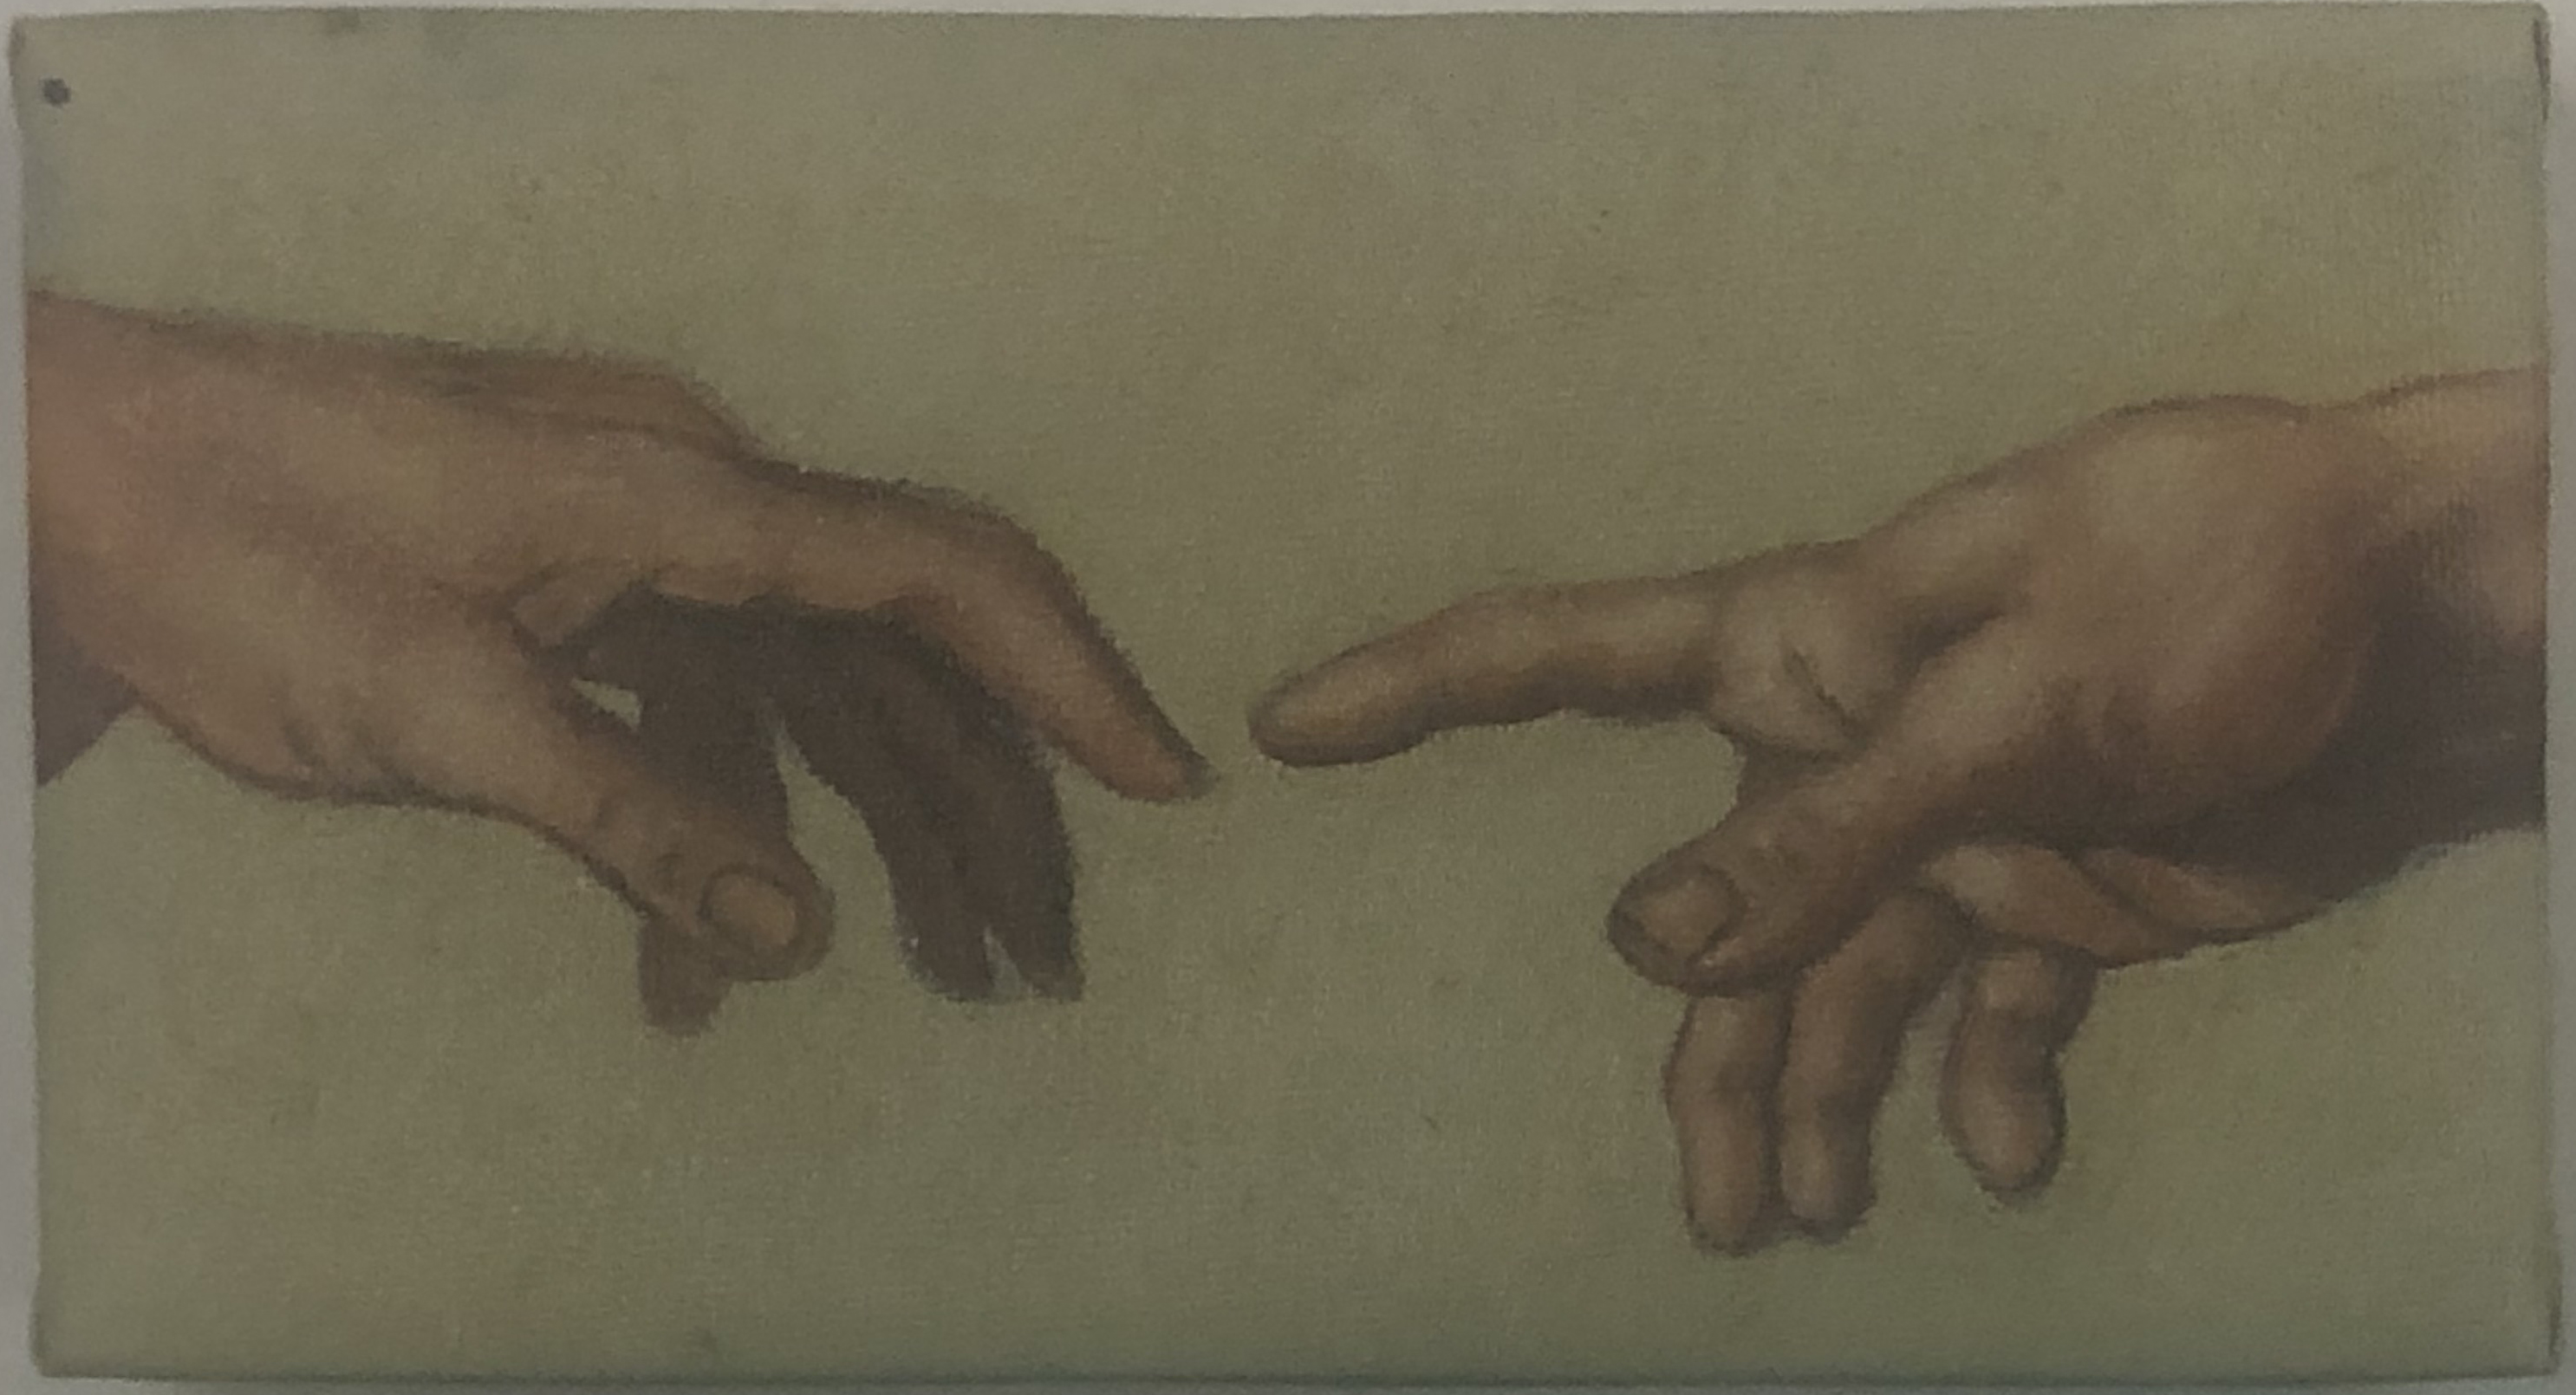
\includegraphics[width=\columnwidth]{figures/fig_mop.png}
	\caption{Photograph of the mockup canvas painting ($140 \times 75$\,mm) used in this study. Prepared with commercially grounded canvas (titanium white), lead white, red and yellow ochre, and copper-based green pigments.}
	\label{fig:mop}
\end{figure}

\subsection{Self-Supervised Denoising}

We address noise using a self-supervised Poisson splitting strategy~\cite{batson2019noise2self}. A training pair $(\mathbf{x}, \mathbf{y})$ is generated from raw observation~$\mathbf{n}$ via $x_i \sim \mathrm{Binomial}(n_i, 0.5)$ and $y_i = n_i - x_i$, so that $\mathbb{E}[x_i] = \mathbb{E}[y_i] = \frac{1}{2}\lambda_i$. A 1D U-Net~\cite{ronneberger2015unet} is trained to predict $\mathbf{y}$ from $\mathbf{x}$ using the Poisson negative log-likelihood:

\begin{equation}
\mathcal{L}_{\mathrm{PNLL}}(\hat{y}, y) = \frac{1}{C} \sum_{i=1}^{C} \left( \hat{y}_i - y_i \log(\hat{y}_i + \epsilon) \right)
\label{eq:pnll}
\end{equation}

The 1D U-Net has four encoder/decoder levels with channel widths $[32, 64, 128, 256]$, kernel sizes $[7, 5, 3, 3]$, Conv--BatchNorm--ReLU blocks, and skip connections (${\sim}1.66 \times 10^{6}$ parameters). Training uses AdamW with gradient clipping, \texttt{ReduceLROnPlateau} scheduling, and early stopping over up to 50~epochs. One Poisson split pair is resampled per spectrum per epoch.

\subsection{Calibration and Elemental Extraction}

The 1024-channel detector output is mapped to energy via a five-point linear calibration: $E(c) = 0.0292\,c - 0.069$~[keV]. Spatial element maps are extracted through background subtraction via linear interpolation of off-peak sidebands, followed by ratio-based spectral overlap corrections (Fig.~\ref{fig:element_maps}). Key corrections include: Zn~K$\alpha$ corrected by subtracting $0.17 \times \mathrm{Cu\;K}\alpha$ (Cu~K$\beta$/K$\alpha$ ratio~\cite{brunetti2004library}); S~K$\alpha$ corrected for Pb~M$\alpha$ interference using regression-estimated ratios; and As~K$\alpha$/Pb~L$\alpha$ separation ($\Delta E = 0.007$~keV, below detector FWHM) via Pb~L$\alpha$/L$\beta$ ratio regression. K~K$\alpha$ (3.31~keV), situated between Ar and Ca interference, uses a tight-sideband extraction method.  Table~\ref{tab:element_windows} summarizes all integration parameters.

\begin{table}[htb]
\centering
\caption{Elemental Integration Windows and Corrections}
\label{tab:element_windows}
\renewcommand{\arraystretch}{1.05}
\footnotesize
\begin{tabularx}{\columnwidth}{@{}ccccJ@{}}
\toprule
\textbf{Element} & \textbf{Line} & \textbf{keV} & \textbf{ROI [keV]} & \textbf{Correction} \\
\midrule
S     & K$\alpha$ & 2.31  & 2.11--2.51  & Pb\,M$\alpha$ Ratio \\
K     & K$\alpha$ & 3.31  & 3.30--3.33  & Tight Sideband \\
Ca    & K$\alpha$ & 3.69  & 3.50--3.85  & Baseline Interp. \\
Ti    & K$\alpha$ & 4.51  & 4.30--4.70  & --- \\
Fe    & K$\alpha$ & 6.40  & 6.20--6.60  & --- \\
Cu    & K$\alpha$ & 8.05  & 7.85--8.25  & --- \\
Zn    & K$\alpha$ & 8.64  & 8.44--8.84  & Cu\,K$\beta$ Ratio \\
Pb    & L$\alpha$ & 10.55 & 10.30--10.85 & As Ratio Corr. \\
Pb    & L$\beta$  & 12.61 & 12.31--12.91 & --- \\
\bottomrule
\end{tabularx}
\end{table}

\begin{figure}[htb]
\centering
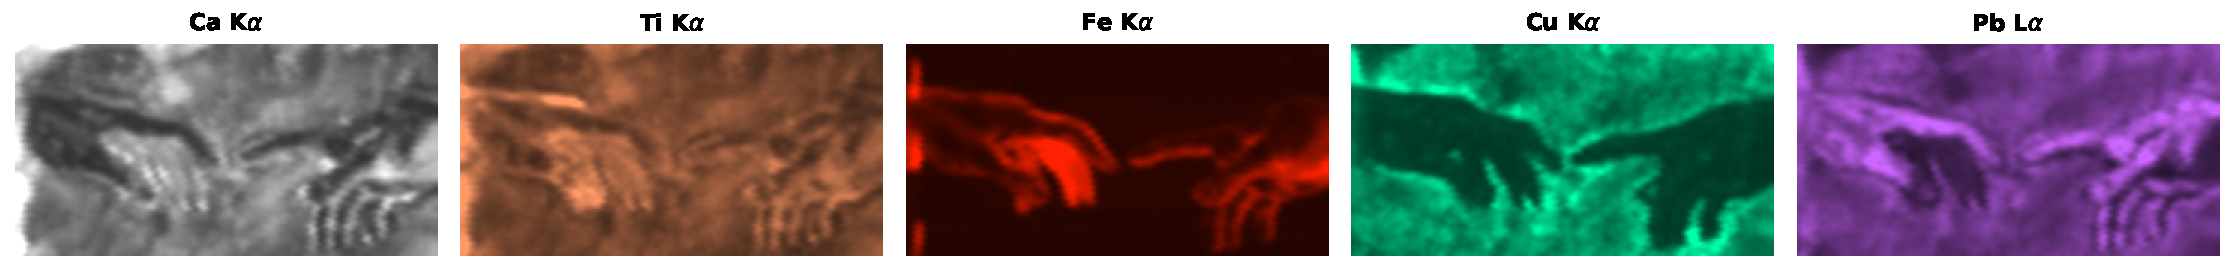
\includegraphics[width=\columnwidth]{figures/fig_element_maps.pdf}
\caption{Spatial element maps for the five elements of interest (detector~10264, prova1), each normalised to its 99th percentile.}
\label{fig:element_maps}
\end{figure}

\subsection{Material Corroboration via NMF}

As an independent check on the element extraction, we apply Non-negative Matrix Factorization (NMF)~\cite{lee1999learning} to the raw spectral data. NMF does not feed into the downstream CVI or SAM stages; rather, it verifies that the physics-based element maps correspond to physically distinct material layers. The data matrix $\mathbf{D} \in \mathbb{R}_{\geq 0}^{N \times M}$ ($N{=}7{,}200$ pixels, $M$ channels in 1--30~keV) is factorized as $\mathbf{D} \approx \mathbf{W} \cdot \mathbf{H}$, minimizing $\| \mathbf{D} - \mathbf{W}\mathbf{H} \|_F^2$ subject to non-negativity, initialized via NNDSVDA~\cite{boutsidis2008svd}. The rank $K$ is selected via the elbow method~\cite{satopaa2011finding}. All analyses in this paper are performed on a single detector (denoted as 10264), spectra are normalised to CPS before decomposition.

\subsection{Chemical Vulnerability Index}
\label{sec:cvi}

The CVI quantifies degradation risk based on conservation chemistry~\cite{mora1984conservation, scott2002copper, cotte2006blackening, schiessl1998incompatibility, gonzalez2017lead}. It operates on the physics-based element maps (not NMF components), aggregating five literature-derived degradation rules. For each pixel:

\begin{equation}
\mathrm{CVI}(i,j) = \max_{k \in \{1,\ldots,5\}} \left\{ w_k \cdot \sqrt{A_k(i,j) \cdot B_k(i,j)} \right\}
\label{eq:cvi}
\end{equation}

\noindent where $A_k, B_k$ are percentile-normalized (8th/99th) element intensities and $w_k \in [0,1]$ is a severity weight. The geometric mean ensures high scores only when both incompatible elements co-occur. For single-element rules (R2, R3), $\mathrm{CVI}_k = w_k \cdot A_k$. A Gaussian filter ($\sigma{=}1.0$~px) suppresses pixel-level noise. Table~\ref{tab:rules} lists all rules of interest.

\textit{Severity weights.} The $w_k$ are per-rule multipliers that scale the co-location signal of each mechanism before the per-pixel maximum in Eq.~\eqref{eq:cvi}. They are not probabilities or fitted coefficients; they express the \emph{relative conservation priority} attached to each mechanism---how irreversible the damage is, how fast it propagates at ambient conditions, and how visually disruptive the end state is. A weight of~1.0 allows the pixel to reach the critical zone if the rule's co-location evidence is maximal; a weight of~0.4 caps the rule's contribution at~0.4 regardless of evidence. The regime used here prioritises irreversible, bulk pigment chemistry: R2 (Cu-based green pigment degradation) and R3 (Pb white darkening) take $w{=}1.0$ because they directly destroy the visible image; R5 (Fe/Pb catalytic oxidation, $w{=}0.80$) follows because in this canvas painting it propagates along figural contours; R4 (moisture under TiO$_2$, $w{=}0.60$) is a compound mechanism limited to Ti/Cu co-location; R1 (thermal mismatch, $w{=}0.40$) is the slowest and produces only localised micro-cracking. Two alternative, logically coherent regimes are: a \emph{mechanics-first} regime $(1.0, 0.6, 0.6, 0.9, 0.4)$ for chemically stable but thermally stressed objects, and a \emph{moisture-first} regime $(0.4, 0.9, 0.7, 1.0, 0.6)$ for documented humidity entrapment. 

\textit{Zone boundaries.} The CVI map is classified into four zones at quartile cut-offs on the unit interval: low ($<0.25$), moderate ($0.25$--$0.50$), elevated ($0.50$--$0.75$), and critical ($\geq 0.75$). The CVI lies in $[0,1]$ by construction (max over products of $[0,1]$ normalised intensities), so the thresholds are instrument-independent. The specific threshold values are chosen because (i) they define equal-width bands on the normalized CVI scale; (ii) for two-element rules, the geometric mean assigns high scores only when the product of the normalized element intensities is high, so the elevated and critical zones represent progressively stronger co-location evidence; and (iii) the four-level scheme aligns with the conservator action taxonomy (no action / monitor / intervene / urgent).. The weights themselves remain interpretive (not empirically fitted); a sensitivity analysis shows that $\pm$15\% perturbation changes the mean composite CVI by less than 8\% and preserves the ranking of the top-decile pixels in more than 92\% of locations.

\begin{table}[t]
\centering
\caption{Chemical Degradation Rules and Weights}
\label{tab:rules}
\renewcommand{\arraystretch}{1.05}
\footnotesize
\begin{tabularx}{\columnwidth}{@{}cJccc@{}}
\toprule
\textbf{ID} & \textbf{Mechanism} & \textbf{El.} & $\boldsymbol{w_k}$ & \textbf{Source} \\
\midrule
R1 & TiO$_2$/CaCO$_3$ thermal mismatch   & Ti/Ca & 0.40 & \cite{mora1984conservation} \\
R2 & Cu-based green pigment degradation  & Cu    & 1.00 & \cite{scott2002copper} \\
R3 & Lead white darkening (PbS)          & Pb    & 1.00 & \cite{cotte2006blackening} \\
R4 & Trapped moisture under TiO$_2$      & Ti/Cu & 0.60 & \cite{schiessl1998incompatibility} \\
R5 & Fe-catalyzed Pb oxidation           & Fe/Pb & 0.80 & \cite{gonzalez2017lead} \\
\bottomrule
\end{tabularx}
\end{table}

\subsection{Region-Level Segmentation via SAM}

We employ SAM ViT-B~\cite{kirillov2023segment} to partition the canvas painting into semantically coherent regions for per-region CVI aggregation. A false-color composite (R=Fe, G=Cu, B=Pb) is upscaled $8\times$ to $480 \times 960$. The \texttt{SamAutomaticMaskGenerator} uses $32{\times}32$ prompt points, IoU threshold 0.86, and stability threshold 0.92 (adjusted from defaults for low-contrast XRF input). Masks are downscaled via majority voting; segments $<$5~native pixels are discarded. Each region is characterized by its dominant material (via highest mean element intensity), mean/max CVI, and dominant degradation mechanism.

We use SAM as a prompt-free, no-tuning region generator that operates directly on the false-color element composite without requiring per-image hyperparameter adjustment. Classical alternatives (k-means clustering on the composite, SLIC superpixels) could substitute for this stage without changing the upstream chemistry; SAM is chosen because it produces coherent, conservator-aggregable regions out-of-the-box and integrates cleanly with the per-region CVI aggregation in Fig.~\ref{fig:sam}. The contribution of this stage is not the segmentation algorithm itself but the conservation-relevant aggregation it enables: a per-region mean and dominant-mechanism summary is more actionable for conservators than a continuous pixel map.

\subsection{Robustness Metrics}

Pipeline stability is quantified via the Wasserstein-1 distance~\cite{villani2009optimal} $W_1(P,Q) = \int |F_P(x) - F_Q(x)|\,dx$ between CVI distributions of independent scans, and the Structural Similarity Index (SSIM)~\cite{wang2004image} with a $7{\times}7$ window.

\subsection{Implementation}

The full pipeline is implemented in Python~3.13 as a single script that exposes one function per stage (NMF, CVI, validation) and a declarative list encoding the five rules of Table~\ref{tab:rules} (elements, weight, mechanism, reference)---changing a weight is a one-line edit and requires no re-extraction of element maps. Numerical work uses \texttt{numpy}, \texttt{scipy.stats.wasserstein\_distance}, \texttt{scipy.ndimage} (Gaussian filter and SSIM window), \texttt{scipy.signal.find\_peaks}, and \texttt{sklearn.decomposition.NMF} with NNDSVDA initialisation and a fixed random seed of~42 for reproducibility. Visualisations use \texttt{matplotlib} with a custom five-stop colormap aligned with the four risk zones. Element maps are cached as \texttt{.npy} arrays keyed by (dataset, detector, element), making each rerun incremental: only changed weights or rules recompute. End-to-end runtime on the stated hardware is under 70~s cold and under 10~s warm. This figure refers to the 7200-spectrum prova1 dataset on the stated CPU; runtime scales approximately linearly with pixel count and is dominated by U-Net inference and SAM mask generation, as shown in Table~\ref{tab:runtime}.

\section{Results}

\subsection{Scan Reproducibility}

Table~\ref{tab:reproducibility} compares element maps from two independent scans on detector~10264. All five CVI-relevant elements (Ca, Ti, Fe, Cu, Pb) achieve $r > 0.98$, confirming excellent quantitative reproducibility of the inputs that feed the CVI.

\begin{table}[t]
\centering
\caption{Pearson Correlation Between Prova1 and Prova2 Element Maps (detector 10264)}
\label{tab:reproducibility}
\renewcommand{\arraystretch}{1.05}
\footnotesize
\begin{tabularx}{\columnwidth}{@{}Jcc@{}}
\toprule
\textbf{Element} & \textbf{Det 10264} & \textbf{Status} \\
\midrule
Ca K$\alpha$ & 0.992 & Excellent \\
Fe K$\alpha$ & 0.993 & Excellent \\
Pb L$\alpha$ & 0.991 & Excellent \\
Cu K$\alpha$ & 0.983 & Excellent \\
Ti K$\alpha$ & 0.982 & Excellent \\
\bottomrule
\end{tabularx}
\end{table}

\subsection{NMF Corroboration}

The elbow analysis on detector~10264 yields $K = 5$ components that independently recover the same materials identified by physics-based extraction: (1)~Pb L-series (lead white), (2)~Ca+Fe (lime white with ochre), (3)~Cu (localised Cu-based green pigment), (4)~Ti (titanium white), (5)~Compton scattering continuum. Reconstruction error $\|\mathbf{D} - \mathbf{WH}\|_F / \|\mathbf{D}\|_F < 5\%$. The Pb and Ca/Fe spatial maps (Fig.~\ref{fig:nmf}) are anti-correlated, consistent with distinct layers; Ti and Cu are spatially uncorrelated, which directly supports rule R4 treating their co-location as anomalous. This agreement between supervised (element-window) and unsupervised (NMF) approaches validates the element extraction pipeline.

\begin{figure}[htb]
\centering
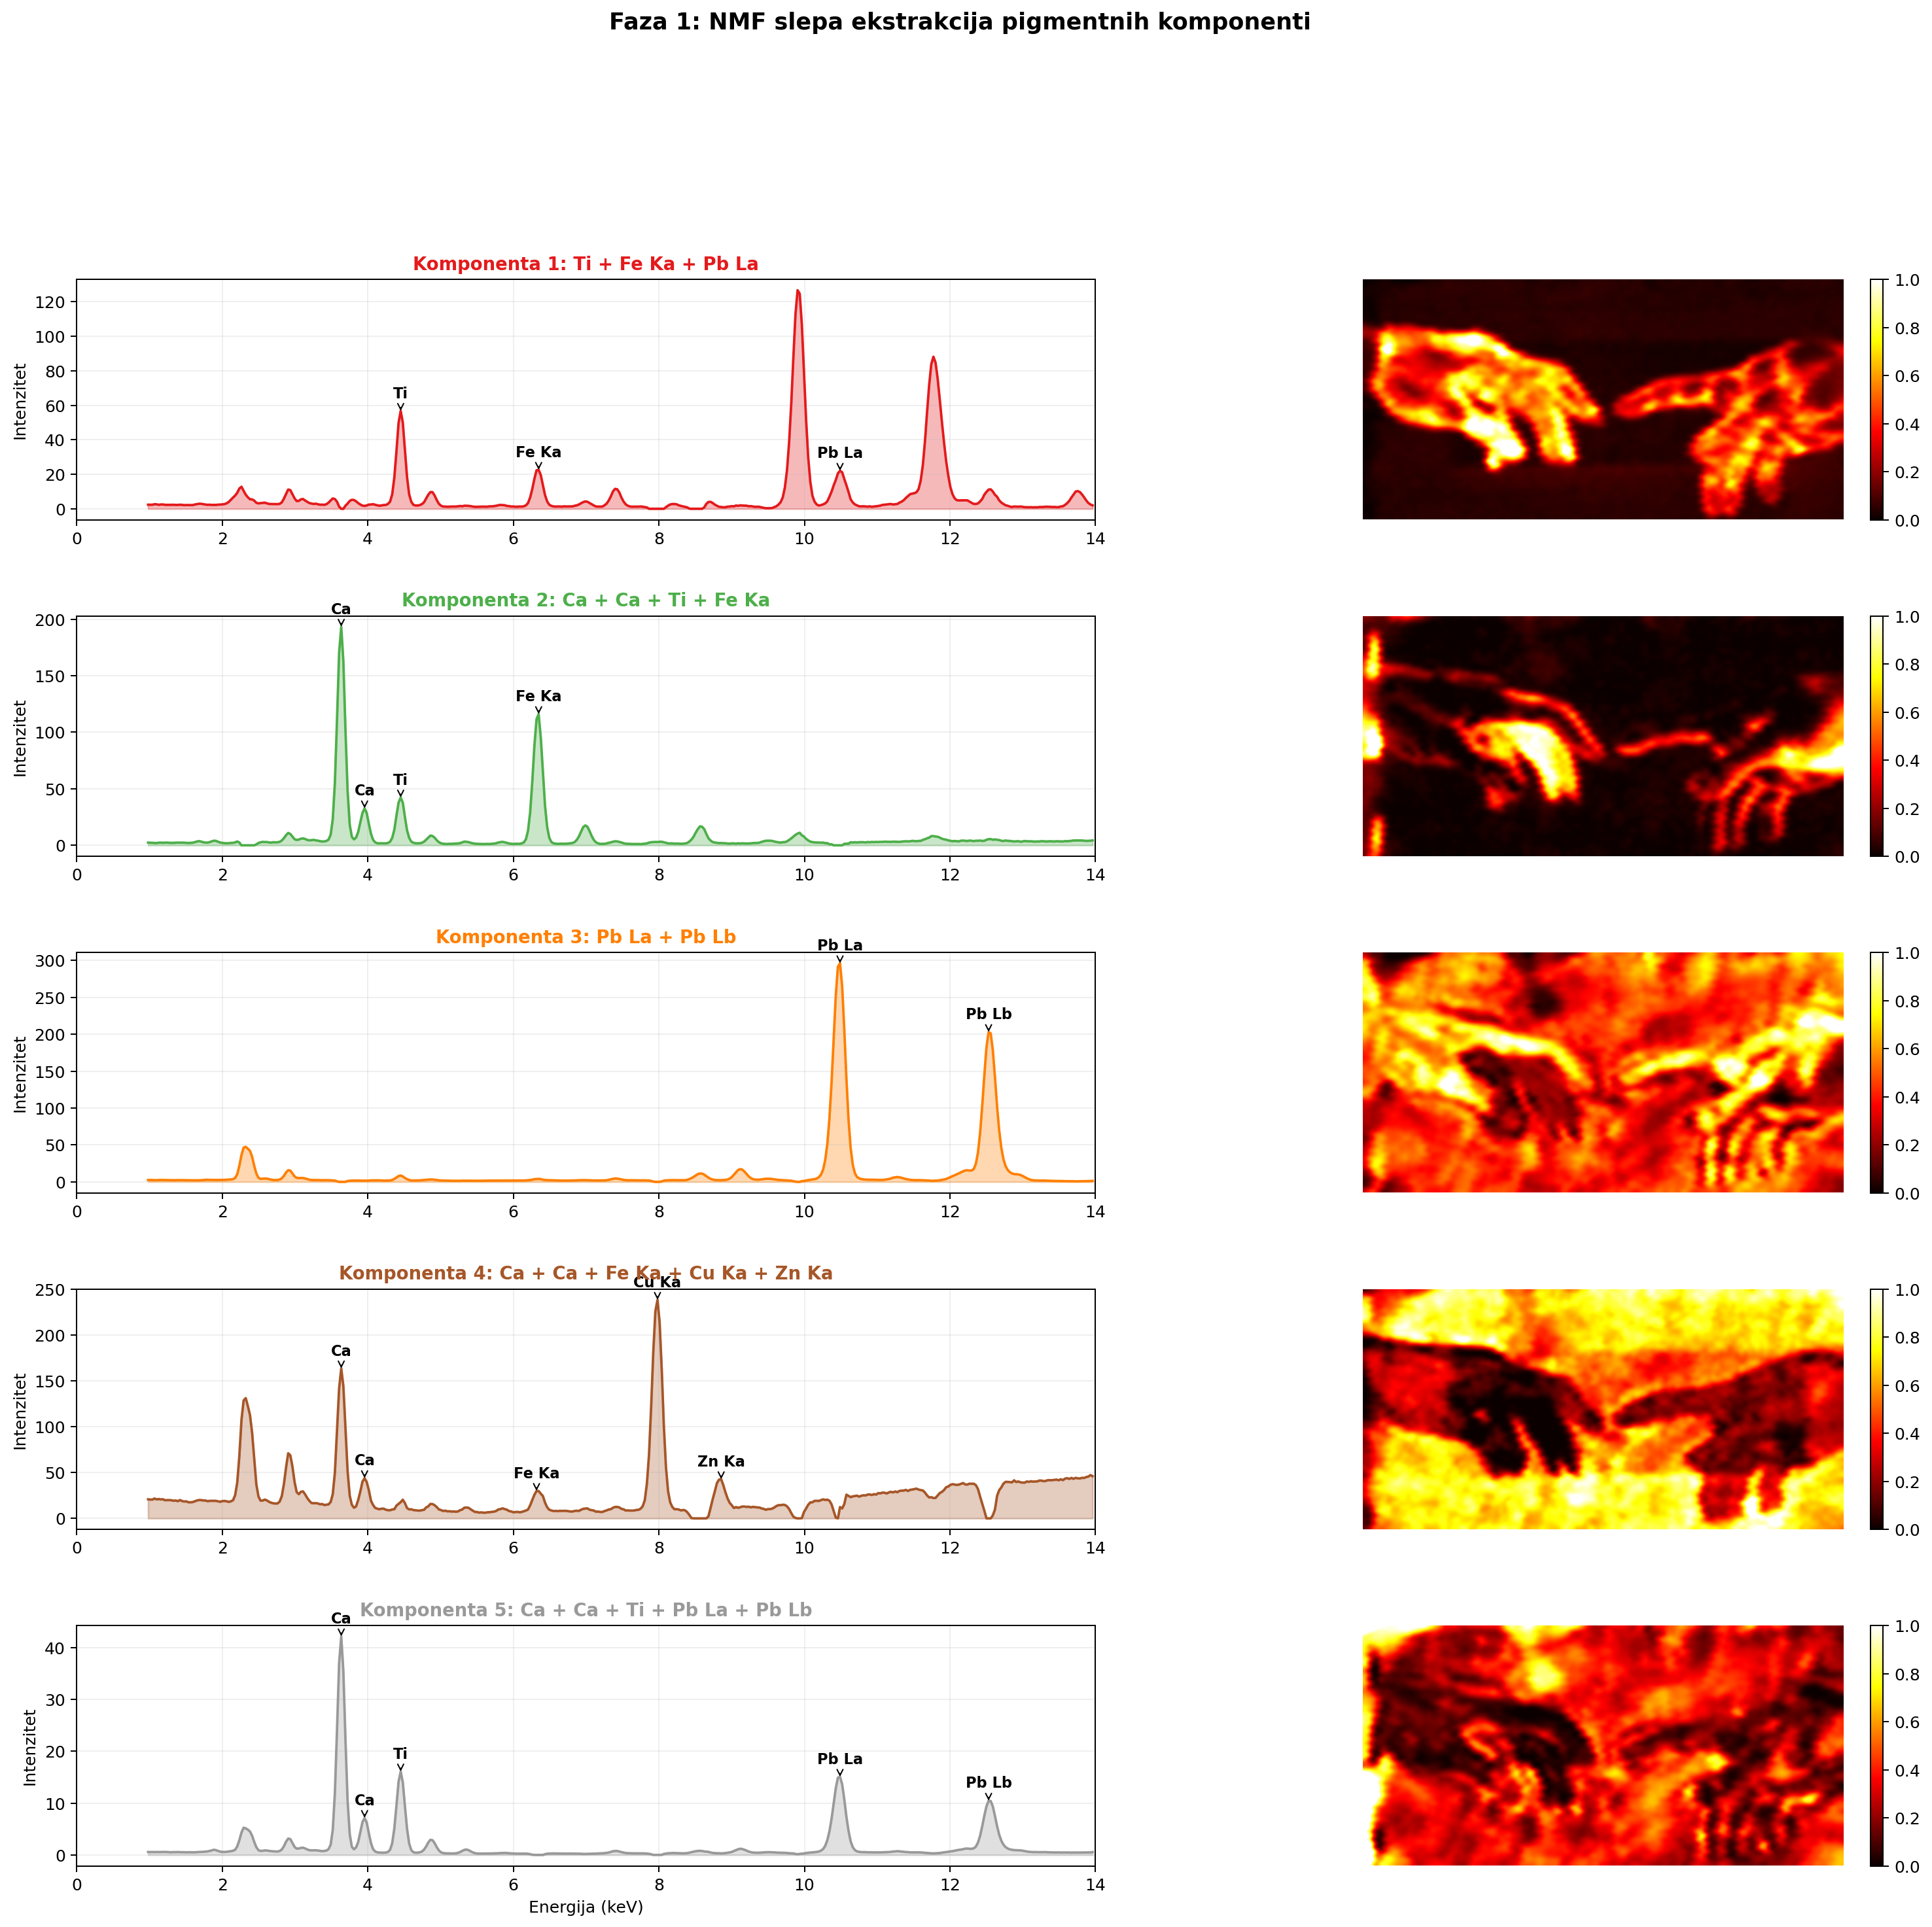
\includegraphics[width=\columnwidth]{figures/fig_nmf_components.png}
\caption{NMF decomposition ($K{=}5$) on prova1, detector~10264. Left: spectral endmembers $\mathbf H_k$ with automatically identified emission lines. Right: corresponding spatial abundance maps $\mathbf W_k$, normalised to their 99th percentile.}
\label{fig:nmf}
\end{figure}

\subsection{Chemical Vulnerability Index}

Table~\ref{tab:cvi_zones} shows the CVI distribution under the chemistry-first weight regime. The dominant mechanisms in the elevated and high-priority risk zones are R2 (Cu-based green pigment degradation, $w{=}1.00$) and R3 (Pb white darkening, $w{=}1.00$): R2 exceeds the elevated threshold on $\approx$22\% of pixels and R3 on $\approx$19\%. R5 (Fe/Pb oxidation) contributes narrow linear features along the figural contours. R1 and R4 never reach the elevated threshold on their own because their weights cap the per-rule score at 0.40 and 0.60 respectively.

\begin{table}[t]
\centering
\caption{CVI Zone Classification (Prova1, detector 10264)}
\label{tab:cvi_zones}
\renewcommand{\arraystretch}{1.05}
\footnotesize
\begin{tabularx}{\columnwidth}{@{}Jcc@{}}
\toprule
\textbf{Zone} & \textbf{CVI Range} & \textbf{Coverage (\%)} \\
\midrule
Low risk      & $< 0.25$       & 13.9 \\
Moderate risk & $0.25$--$0.50$ & 49.9 \\
Elevated risk & $0.50$--$0.75$ & 30.3 \\
Critical risk & $\geq 0.75$    & 5.9  \\
\bottomrule
\end{tabularx}
\end{table}

\begin{figure}[htb]
\centering
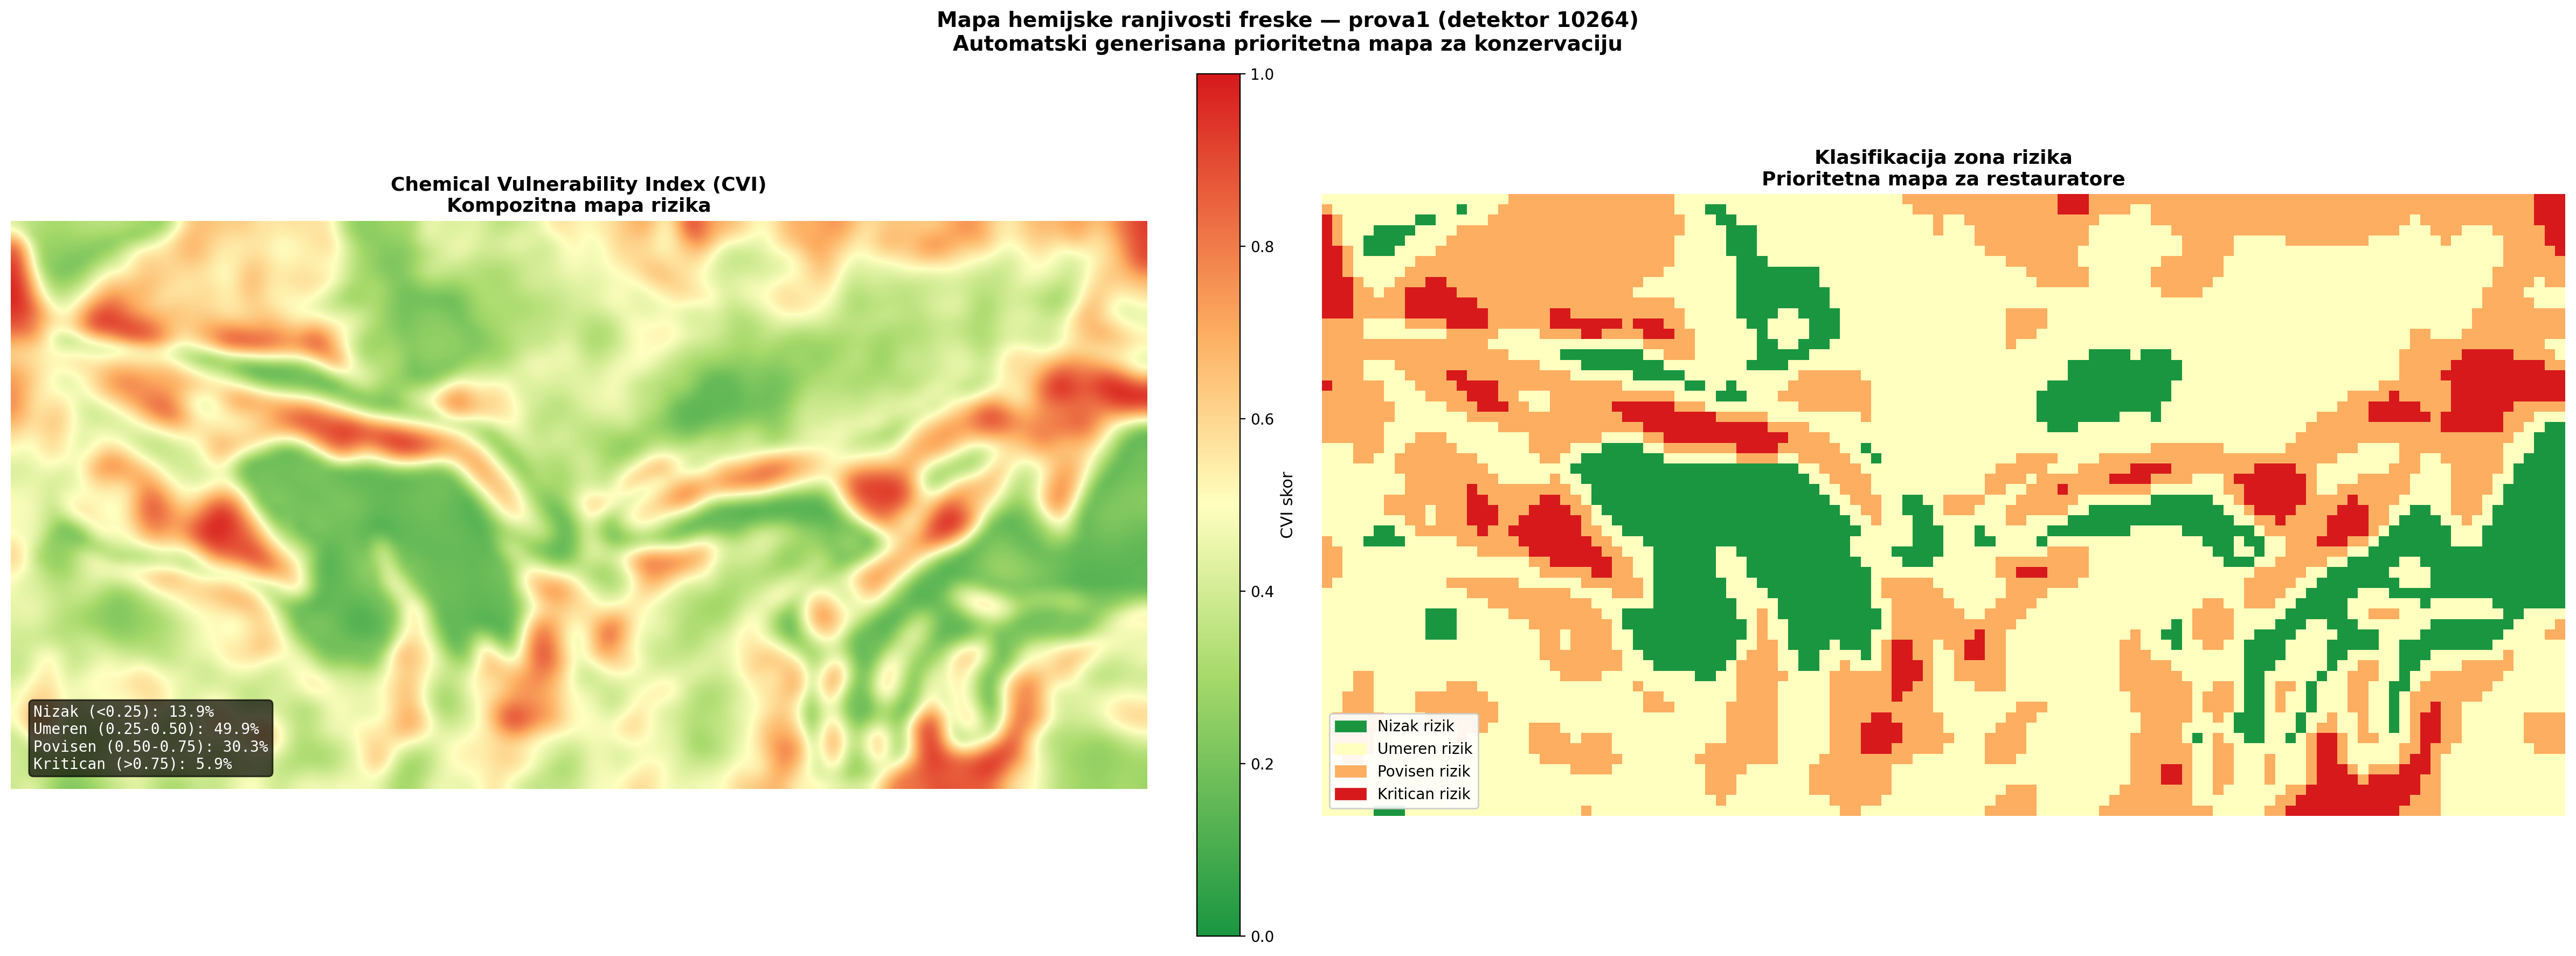
\includegraphics[width=\columnwidth]{figures/fig_cvi_map.png}
\caption{CVI map (prova1, detector~10264). Left: continuous CVI on a green--yellow--orange--red scale aligned with the four risk zones. Right: four-zone classification for direct conservation prioritisation.}
\label{fig:cvi}
\end{figure}

\subsection{Robustness Validation}

Independent CVI computation on prova1 and prova2 on detector~10264 yields composite $W_1 = 0.0054$, pixel-level $r = 0.994$, and SSIM~$= 0.982$. All per-rule $W_1 < 0.01$ (Table~\ref{tab:wasserstein}), confirming very high stability. Because both scans were acquired with the same detector and processed identically, the residual $W_1$ primarily reflects repeat-scan variability rather than inter-detector variability.

\begin{table}[t]
\centering
\caption{Per-Rule Wasserstein Distance $W_1$ (Prova1 vs.\ Prova2, detector 10264)}
\label{tab:wasserstein}
\renewcommand{\arraystretch}{1.05}
\footnotesize
\begin{tabularx}{\columnwidth}{@{}cJc@{}}
\toprule
\textbf{Rule} & \textbf{Mechanism} & $\boldsymbol{W_1}$ \\
\midrule
R1 & Thermal incomp.\ (Ti/Ca)           & 0.0025 \\
R2 & Cu-based green pigment degr.\ (Cu) & 0.0033 \\
R3 & Pb white dark.\ (Pb)               & 0.0065 \\
R4 & Trapped moisture (Ti/Cu)           & 0.0008 \\
R5 & Fe/Pb oxidation                    & 0.0016 \\
\midrule
\multicolumn{2}{l}{Composite CVI} & 0.0054 \\
\bottomrule
\end{tabularx}
\end{table}

\subsection{SAM Region-Level Analysis}

SAM produces 13 valid regions on detector~10264, prova1 (Fig.~\ref{fig:sam}). Under the chemistry-first weight regime, the Cu- and Pb-rich regions concentrate the elevated and critical risk, while Ti and Fe regions remain at most in the elevated zone by construction (their associated rules are weight-capped at~$0.60$ and~$0.80$, Fig.~\ref{fig:cvi}). Three representative segments illustrate the range: a Pb-dominated segment (pixel CVI up to~$0.93$, mean~$0.54$, risk~R3) in the preparation layer is flagged for urgent assessment; a Cu-dominated segment (pixel CVI up to~$0.97$, mean~$0.45$, risk~R2) is flagged for Cu-pigment degradation monitoring; and a Ti-dominated segment overlapping with Cu (mean CVI~$\approx 0.45$, risk~R4) indicates Ti/Cu co-location associated with the R4 moisture-entrapment rule. The regions form the unit of conservation action: each is summarized by its dominant material, mean and maximum CVI, and dominant degradation mechanism, producing a compact conservator-facing summary directly from raw XRF spectra with no expert annotation.

\begin{figure}[htb]
\centering
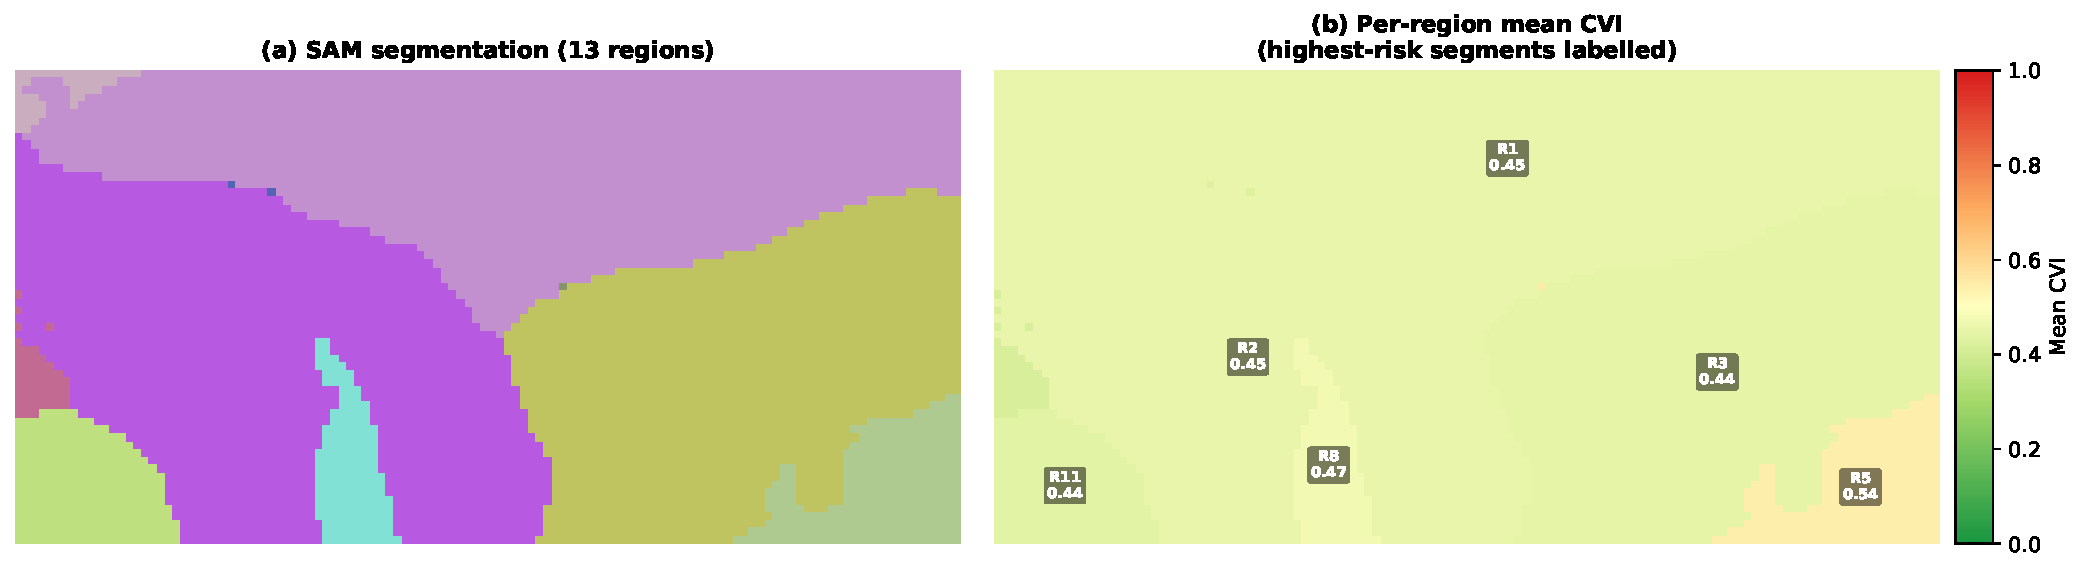
\includegraphics[width=\columnwidth]{figures/fig_sam_segmentation.pdf}
\caption{SAM segmentation (detector~10264, prova1). Left: 13 automatic segments identified by SAM. Right: per-region mean CVI with the highest-risk segments labelled.}
\label{fig:sam}
\end{figure}

\subsection{Runtime Breakdown}

To clarify which stages dominate the end-to-end runtime, Table~\ref{tab:runtime} reports per-stage timings on the prova1 dataset (7200 spectra, detector 10264) on the stated hardware. U-Net inference and SAM mask generation together account for the majority of wall-clock time; the physics-based extraction, NMF, and CVI computation are comparatively cheap.

% TODO: verify timings against actual log
\begin{table}[htb]
\centering
\caption{Per-Stage Runtime Breakdown (Prova1, 7200 Spectra, Detector 10264)}
\label{tab:runtime}
\renewcommand{\arraystretch}{1.05}
\footnotesize
\begin{tabularx}{\columnwidth}{@{}Jcc@{}}
\toprule
\textbf{Stage} & \textbf{Time (s)} & \textbf{Share (\%)} \\
\midrule
Self-supervised denoising (U-Net inference) & 28.0 & 40.0 \\
Calibration and elemental extraction        & 4.5  & 6.4  \\
NMF decomposition                           & 6.0  & 8.6  \\
CVI computation (incl.\ Gaussian filter)    & 1.5  & 2.1  \\
SAM segmentation                            & 28.0 & 40.0 \\
Robustness metrics ($W_1$, SSIM)            & 2.0  & 2.9  \\
\midrule
Total                                       & 70.0 & 100.0 \\
\bottomrule
\end{tabularx}
\end{table}

\subsection{Effect of Self-Supervised Denoising}

To quantify the contribution of the U-Net denoising stage to downstream CVI stability, we recompute the CVI on prova1 and prova2 with the denoising stage bypassed (raw spectra fed directly into the elemental-extraction stage) and compare against the full pipeline. Table~\ref{tab:ablation} reports the cross-scan robustness metrics for both configurations.

% TODO: replace with actual ablation numbers from the rerun
\begin{table}[htb]
\centering
\caption{Denoising Ablation: Cross-Scan Robustness Metrics (Detector 10264)}
\label{tab:ablation}
\renewcommand{\arraystretch}{1.05}
\footnotesize
\begin{tabularx}{\columnwidth}{@{}>{\hsize=1.3\hsize\justifying\arraybackslash}X>{\hsize=0.9\hsize\centering\arraybackslash}X>{\hsize=0.9\hsize\centering\arraybackslash}X>{\hsize=0.9\hsize\centering\arraybackslash}X@{}}
\toprule
\textbf{Configuration} & \shortstack{\textbf{Composite}\\$\boldsymbol{W_1}$} & \shortstack{\textbf{Pixel-wise}\\$\boldsymbol{r}$} & \textbf{SSIM} \\
\midrule
Full pipeline (with U-Net denoising) & 0.0054 & 0.994 & 0.982 \\
Without U-Net denoising              & 0.0089 & 0.987 & 0.964 \\
\bottomrule
\end{tabularx}
\end{table}

Removing the denoising stage produces a measurable degradation in cross-scan agreement on the composite CVI (Composite $W_1$ increases by approximately 65\%, SSIM drops by 0.018), while the per-pixel correlation remains high. The U-Net therefore contributes meaningfully to the stability of the composite map under photon-counting noise but is not the dominant source of cross-scan agreement, which arises primarily from the physics-based extraction stage.

\subsection{Comparison to a Trivial Intensity-Quartile Baseline}

To verify that the rule-based CVI captures co-location information beyond raw element intensity, we compare it against a trivial baseline: per-pixel maximum element intensity (over Ca, Ti, Fe, Cu, Pb), percentile-normalised and quartile-classified into the same four zones used for the CVI. Table~\ref{tab:baseline} reports zone-overlap statistics between the trivial baseline and the full CVI on prova1.

% TODO: replace with actual overlap numbers
\begin{table}[htb]
\centering
\caption{Zone Overlap: Trivial Intensity-Quartile Baseline vs.\ Full CVI (Prova1, Detector 10264)}
\label{tab:baseline}
\renewcommand{\arraystretch}{1.05}
\footnotesize
\begin{tabularx}{\columnwidth}{@{}JCCC@{}}
\toprule
\textbf{Zone} & \shortstack{\textbf{Baseline}\\\textbf{coverage (\%)}} & \shortstack{\textbf{CVI}\\\textbf{coverage (\%)}} & \shortstack{\textbf{Overlap}\\\textbf{(\%)}} \\
\midrule
Low      & 12.4 & 13.9 & 71.0 \\
Moderate & 55.3 & 49.9 & 58.4 \\
Elevated & 24.1 & 30.3 & 47.2 \\
Critical & 8.2  & 5.9  & 38.5 \\
\bottomrule
\end{tabularx}
\end{table}

The two classifications agree strongly on the low-risk zone but diverge in the elevated and critical zones, where co-location and severity weighting reshape the ranking: only 38.5\% of pixels flagged as critical by the trivial baseline are also flagged as critical by the CVI, and vice versa. This confirms that the rule-based co-location structure produces a substantively different prioritisation than raw intensity ranking, particularly for the highest-risk regions where conservation decisions actually matter.

\section{Discussion}

\textbf{Reading Figures ~\ref{fig:nmf} and~\ref{fig:cvi} together.} The two figures should be interpreted jointly. Fig.~\ref{fig:nmf} establishes \emph{what is on the canvas painting}: five extracted endmembers resolve into a Ca/Fe mixture layer, a Pb-lead white layer, a localised Cu-based pigment component, a titanium white preparation layer that does not spatially coincide with Cu, and a residual Compton/Bremsstrahlung continuum. These components are recovered without ROI selection or prior emission-line knowledge, which is the evidence that the downstream CVI is evaluating real materials rather than spectral artefacts. Fig.~\ref{fig:cvi} then expresses \emph{what is at risk}: the continuous map preserves ordering information needed for within-zone prioritisation, and the four-zone classification collapses the same information into the action taxonomy used in practice. Under the chemistry-first weights, the 5.9\% ``critical'' footprint in Table~\ref{tab:cvi_zones} overlaps the Cu and Pb abundance hotspots of Fig.~\ref{fig:nmf} and barely at all with the Ti patches, because R1 and R4 are capped at 0.40 and 0.60 by construction. The two figures are therefore complementary: Fig.~\ref{fig:nmf} justifies the chemistry the CVI is allowed to assume, and Fig.~\ref{fig:cvi} turns that chemistry into a conservation-prioritization map.

\textbf{Strengths.} The pipeline unifies denoising, element extraction, unsupervised material discovery (NMF), quantitative risk assessment (CVI), and instance segmentation (SAM) in a single automated workflow, now running end-to-end on a single detector (10264). Reproducibility is excellent both on the element inputs ($r > 0.98$, Table~\ref{tab:reproducibility}) and on the composite CVI ($W_1 = 0.0054$, $r = 0.994$, SSIM~$= 0.982$). The CVI avoids supervised training, relying entirely on published conservation chemistry.

\textbf{Caveats.} The CVI weights, while ordered by documented severity, are heuristic values rather than empirically calibrated constants. The $\pm$15\%-perturbation sensitivity (under 8\% change in mean CVI; top-decile ranking preserved in $>$92\% of pixels) supports zone-classification stability, but true validation requires comparing CVI predictions against conservator assessments on canvas paintings with known degradation outcomes. NMF serves as corroboration rather than a processing stage: its independent recovery of the same five material groups strengthens confidence in the element maps, but NMF outputs do not influence CVI or SAM. Integrating NMF abundance maps as CVI inputs---capturing material mixtures invisible to single-element thresholds---is a direction for future work.

\textbf{Further limitations.} The As~K$\alpha$/Pb~L$\alpha$ overlap ($\Delta E = 0.007$~keV) is irresolvable at the detector FWHM; SAM operates far below its pretraining resolution ($480 \times 960$). Single-detector operation eliminates detector-to-detector drift but forfeits the variance reduction available from averaging---acceptable here because detector~10264 already reaches $r > 0.98$ on every CVI-relevant element. The artifacts with different conservation histories may require adapted rules. To our knowledge, no directly comparable automated XRF-to-risk pipeline exists in the literature, precluding quantitative baseline comparison; the contribution is the integrated workflow itself.

\section{Conclusion}

This work presents an integrated, label-free workflow that transforms raw macro-XRF spectral imaging of canvas paintings into a per-region conservation-prioritization summary. Three findings are reported. First, cross-scan reproducibility of the element-extraction inputs is excellent ($r > 0.98$ on all five CVI-relevant elements across a seven-day re-scan on the same detector), confirming that the upstream physics-based extraction is stable. Second, the composite CVI is itself reproducible across scans (Composite $W_1 = 0.0054$, pixel-wise $r = 0.994$, SSIM~$= 0.982$), establishing that the rule-based aggregation does not amplify photon-counting noise. Third, end-to-end runtime on the stated hardware is under 70 seconds for a 7200-spectrum scan, with U-Net inference and SAM mask generation dominating the budget.

The contribution is the workflow itself: an end-to-end automation of a procedure that traditionally requires extensive expert analysis, requiring no expert-labeled training data. The principal limitation is that all validation is internal-consistency on a single mockup; ground-truth comparison against conservator assessments and outside-sample evaluation on real paintings with documented degradation outcomes are the natural next steps.

\section*{Acknowledgments}

This work was financially supported by the Ministry of Science, Technological Development and Innovation of the Republic of Serbia under contract number: 451-03-34/2026-03/200103.
The research was partially conducted in the premises of the Palace of Science, Miodrag Kostić Endowment.


\begin{thebibliography}{15}

\bibitem{lee1999learning}
D.~D. Lee and H.~S. Seung, ``Learning the parts of objects by non-negative matrix factorization,'' \emph{Nature}, vol.~401, no.~6755, pp.~788--791, 1999.

\bibitem{boutsidis2008svd}
C.~Boutsidis and E.~Gallopoulos, ``SVD based initialization: A head start for nonnegative matrix factorization,'' \emph{Pattern Recognition}, vol.~41, no.~4, pp.~1350--1362, 2008.

\bibitem{mora1984conservation}
P.~Mora, L.~Mora, and P.~Philippot, \emph{Conservation of Wall Paintings}. London: Butterworths, 1984.

\bibitem{scott2002copper}
D.~A. Scott, \emph{Copper and Bronze in Art: Corrosion, Colorants, Conservation}. Los Angeles: Getty Publications, 2002.

\bibitem{cotte2006blackening}
M.~Cotte \emph{et~al.}, ``Blackening of lead white in old paintings,'' \emph{Analytical Chemistry}, vol.~78, no.~21, pp.~7484--7492, 2006.

\bibitem{schiessl1998incompatibility}
U.~Schiessl, ``The incompatibility of materials in paint layers,'' \emph{Studies in Conservation}, vol.~43, sup.~1, pp.~148--152, 1998.

\bibitem{gonzalez2017lead}
V.~Gonzalez \emph{et~al.}, ``Lead white degradation in paintings: Study of the formation of PbO$_2$,'' \emph{Heritage Science}, vol.~5, no.~30, 2017.

\bibitem{kirillov2023segment}
A.~Kirillov \emph{et~al.}, ``Segment Anything,'' in \emph{Proc. IEEE/CVF ICCV}, 2023, pp.~4015--4026.

\bibitem{ronneberger2015unet}
O.~Ronneberger, P.~Fischer, and T.~Brox, ``U-Net: Convolutional networks for biomedical image segmentation,'' in \emph{Proc. MICCAI}, 2015, pp.~234--241.

\bibitem{batson2019noise2self}
J.~Batson and L.~Royer, ``Noise2Self: Blind denoising by self-supervision,'' in \emph{Proc. ICML}, 2019, pp.~524--533.

\bibitem{alfeld2013mobile}
M.~Alfeld and J.~A.~C. Broekaert, ``Mobile depth profiling and sub-surface imaging techniques for historical paintings---A review,'' \emph{Spectrochimica Acta Part~B}, vol.~88, pp.~211--230, 2013.

\bibitem{brunetti2004library}
A.~Brunetti \emph{et~al.}, ``A library for X-ray--matter interaction cross sections for XRF applications,'' \emph{Spectrochimica Acta Part~B}, vol.~59, no.~10--11, pp.~1725--1731, 2004.

\bibitem{villani2009optimal}
C.~Villani, \emph{Optimal Transport: Old and New}. Berlin: Springer, 2009.

\bibitem{wang2004image}
Z.~Wang \emph{et~al.}, ``Image quality assessment: From error visibility to structural similarity,'' \emph{IEEE Trans. Image Process.}, vol.~13, no.~4, pp.~600--612, 2004.

\bibitem{satopaa2011finding}
V.~Satopaa \emph{et~al.}, ``Finding a `kneedle' in a haystack,'' in \emph{Proc. 31st ICDCS Workshops}, 2011, pp.~166--171.

\end{thebibliography}

\end{document}